\documentclass[paper=a4, pagesize, twoside, openright, draft=false,
BCOR7mm, DIV13, fontsize=11pt, headings=normal, footinclude=false, 
chapterprefix = false, toc=listof, ngerman, parskip=half]{scrartcl} % doppelseitiger Druck

%%%%%%%%%%%%%%%%%%%%%%%%%%%%%%%%%%%%%%%%%%%%%%%%%%%%%%%%%%%%%%%%%%%%%%%%%%%%%%%%%%%%%%%%%
%%%%%%%%%%%%%%%%%%%%%%%%%%%%%%%%%%%%%%%%%%%%%%%%%%%%%%%%%%%%%%%%%%%%%%%%%%%%%%%%%%%%%%%%
\usepackage{D:/Daten/tex/dsvFPGA_ueb_style_v3}
%%%%%%%%%%%%%%%%%%%%%%%%%%%%%%%%%%%%%%%%%%%%%%%%%%%%%%%%%%%%%%%%%%%%%%%%%%%%%%%%%%%%%%%%
%
%\includeonly{2010-DSP_FPGA-Ueb_Kap_1_2}
%
\hypersetup{
pdftitle={pyFDA: Software Architecture and API},
                   pdfauthor={Christian Muenker},
                   pdfsubject={pyFDA},
                   pdfkeywords={pyFDA, filter design, python}
                   }
\def\CodePath{../pyFDA}
\def\pyFirstLine{1}
%
%
\begin{document}
%\renewmdenv[linecolor=red,frametitle={Wichtige Begriffe}]{infobox}

%\frontmatter
%%%%%%%%%%%%%%%%%%%%%%%%%%%%%%%%%%%%%%%%%%%%%%%%%%%%%%%%%%%%%%%%%%%%%%%%%%%%%%%%%%%%%%%%%
%%%%%%%%%%%%%%%%%%%%%%%%%%%%%%%%%%%%%%%%%%%%%%%%%%%%%%%%%%%%%%%%%%%%%%%%%%%%%%%%%%%%%%%%%
\author{Prof. Dr. Christian M�nker}
\title{pyFDA: Software Architecture and API}
\date{\today}
%\maketitle
\begin{titlepage}
\begin{center}
\begin{Huge}pyFDA: Software Architecture and API\end{Huge}
\\[1cm]
\LARGE Christian M\"unker
\vfill
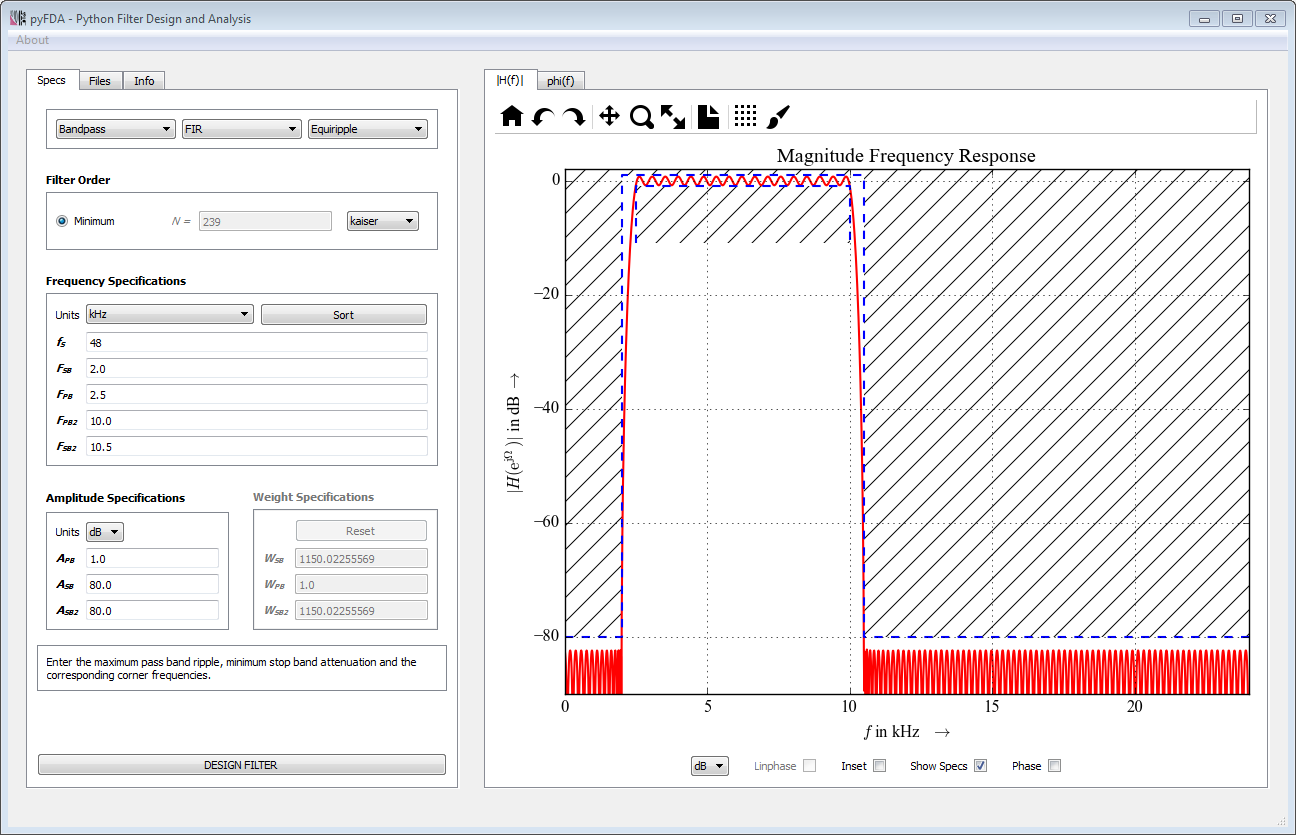
\includegraphics[width=13cm]{pyFDA_screenshot}%{scipy_logo}%{D:/Daten/tex/graphics/IIR_ellip_H_z.png}\\

\footnotesize{Overview}
\vfill
\Large \today \\[1cm]
\href{mailto:Christian.Muenker@hm.edu}{Christian.Muenker@hm.edu}
\end{center}
\end{titlepage}

%
%***********************************************************************%
%*******               TABLE OF CONTENTS                        ********%
%***************                                        ****************%
\clearpage
\phantomsection % needed for correct TOC and hyperlinks
\tableofcontents
\addcontentsline{toc}{section}{Inhaltsverzeichnis}

%
%\def\thesection{\arabic{chapter}.\arabic{section}} 
%\include{DSP_FPGA-Ueb_Changes}
%\addcontentsline{toc}{chapter}{�nderungen}

%\def\thesection{Aufgabe \arabic{chapter}.\arabic{section}} 

%\setcounter{lofdepth}{2} % List of figures mit subfigures


%%%%%%%%%%%%%%%%%%%%%%%%%%%%%%%%%%%%%%%%%%%%%%%%%%%%%%%%%%%%%
\setcounter{topnumber}{3} % max. Anzahl von Gleitobjekten im oberen Teil der Seite

\section{Overview}

\section{Input Widgets}

\section{Plot Widgets}

\section{Filter Objects}
A new filter objects \texttt{my\_filter.py} can be added easily to an pyFDA installation by 

\begin{itemize}
\item copying it to the \texttt{filter\_widgets} directory
\item adding a line with the filename to the list of filter files \texttt{Init.txt} in the same directory.
\end{itemize}

When starting pyFDA, \texttt{filter\_tree\_builder.py} is run, extracting the relevant information and building a hierachical tree in \texttt{filter\_broker.py}. 

The structure of a filter file and the attributes and methods that need to be provided are described in this section.

\subsection{Who needs you?}
A filter design object is instantiated dynamically every time the filter design method is changed in 

\texttt{input\_widgets/input\_filter.py} in \textbt{SelectFilter.setDesignMethod()}

The handle to this object is stored in \texttt{filterbroker.py} in \texttt{filObj}.

The actual design methods (LP, HP, ...) are called dynamically in \texttt{input\_widgets/input\_specs.py} in \textbt{InputSpecs.startDesignFilt()}.

An example for a design method is
\begin{lstlisting}[style = pyStyle]{}
def LPman(self, fil_dict):
	self.get_params(fil_dict)
	self.save(fil_dict, sig.ellip(self.N, self.A_PB, self.A_SB, self.F_PB, 
		btype='low', analog = False, output = frmt))
\end{lstlisting}

with the single parameter \texttt{fil\_dict}, that supplies the global filter dictionary containing all parameters and the designed filter as well. 

The local helper function \texttt{get\_params()} extracts parameters from the global filter dictionary and scales the parameters if required (as in the case for ellip routines):

\begin{lstlisting}[style = pyStyle]{}
def get_params(self, fil_dict):
 """
 Translate parameters from the passed dictionary to instance
 parameters, scaling / transforming them if needed.
 """
 self.N     = fil_dict['N']
 self.F_PB  = fil_dict['F_PB'] * 2 # Frequencies are normalized to f_Nyq
\end{lstlisting}

The local helper function \texttt{save()} saves the filter design back to the dictionary and the filter order and corner frequencies if they have been calculated by a minimum order algorithm.

\begin{lstlisting}[style = pyStyle]{}
def save(self, fil_dict, arg):
  """
  Store results of filter design in the global filter dictionary. Corner
  frequencies calculated for minimum filter order are also stored in the 
  dictionary to allow for a smooth manual filter design.
  """
  pyfda_lib.save_fil(fil_dict, arg, frmt, __name__)

  if self.F_PBC is not None: # has corner frequency been calculated?
    fil_dict['N'] = self.N # yes, update filterbroker
    if np.isscalar(self.F_PBC): # HP or LP - a single corner frequency
      fil_dict['F_PBC'] = self.F_PBC / 2.
    else: # BP or BS - two corner frequencies (BP or BS)
      fil_dict['F_PBC'] = self.F_PBC[0] / 2.
      fil_dict['F_PBC2'] = self.F_PBC[1] / 2.
\end{lstlisting}

The method

\subsection{Info strings}
All information that is displayed in \texttt{input\_widget/input\_info.py} in a \texttt{QtGui.QTextBrowser()} widget is provided in the multi line strings \textbt{self.info} and \textbt{self.info\_doc} in MarkDown format. They are analyzed and converted to HTML using \texttt{publish\_string} from \texttt{docutils.core}. \texttt{self.info} contains self-written information on the filter design method, \texttt{self.info\_doc} optionally collects python docstrings. See an excerpt from \texttt{ellip.py}:
 
\begin{lstlisting}[style=pyStyle]{}
self.info = """
**Elliptic filters**

(also known as Cauer filters) have a constant ripple :math:`A_PB` resp.
:math:`A_SB` in both pass- and stopband(s).

For the filter design, the order :math:`N`, minimum stopband attenuation
:math:`A_SB`, the passband ripple :math:`A_PB` and
the critical frequency / frequencies :math:`F_PB` where the gain drops below
:math:`-A_PB` have to be specified.

**Design routines:**

``scipy.signal.ellip()``
``scipy.signal.ellipord()``
"""

self.info_doc = []
self.info_doc.append('ellip()\n========')
self.info_doc.append(sig.ellip.__doc__)
self.info_doc.append('ellipord()\n==========')
self.info_doc.append(ellipord.__doc__)
\end{lstlisting}


\end{document}
